\documentclass[14pt, a4paper]{article}
\usepackage[utf8]{inputenc}
\usepackage{graphicx}
\usepackage[portuguese]{babel}
\usepackage{natbib}


\title{MA531- ALGEBRA VETORIAL E LINEAR PARA COMPUTAÇÃO}
\author{Maria Clara Albuquerque Moura}
\date{Setembro, 2022}

\begin{document}

\maketitle
\section{Introdução da Disciplina}
\label{sec:introducao}

\paragraph{}

Álgebra Vetorial e Linear para Computação \citep{MA531} é uma disciplina da graduação em Ciência da Computação e, entre seus objetivos, está a capacitação dos discentes mediante a exposição dos princípios fundamentais da álgebra matricial e vetorial, tais como: transformações lineares e espaços vetoriais, estruturas matriciais e medidas em espaços vetoriais. Alinhado ao ensino desses tópicos, são expostas técnicas de demonstração de teoremas, bem como a apresentação de aplicações motivadoras dos assuntos em questão.

\begin{figure}[ht]
\centering
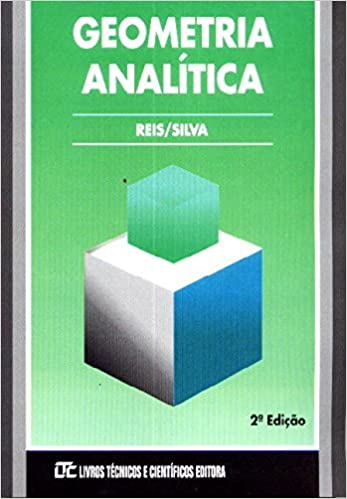
\includegraphics[width=5cm]{images/g.analitica.jpg}
\caption{Geometria Analítica - Reis e Silva - LTC}
\label{figura:geometria}
\end{figure}

\begin{figure}[ht]
\centering
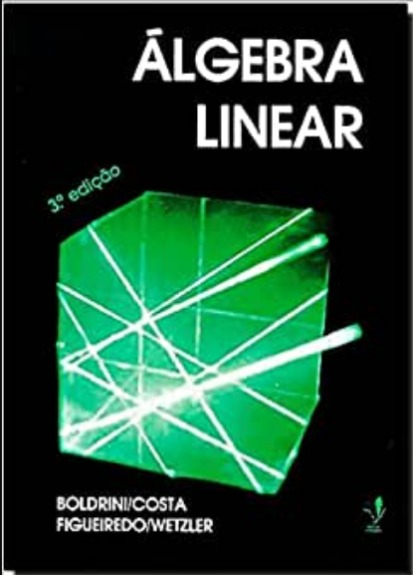
\includegraphics[width=5cm]{images/a.linear.jpeg}
\caption{Algebra Linear - Boldrini/Costa/ Figueiredo/Wetzler - Harbra.}
\label{figura:algebra}
\end{figure}

\paragraph{}

Os livros destacados nas Figuras \ref{figura:geometria} e \ref{figura:algebra} são utilizados como bibliografia complementar aos conceitos estudados durante a disciplina, de forma a expandir a base teórica e obter exercícios adicionais que facilitem a compreensão do objeto de estudo.

\paragraph{}

No prefácio do livro  Álgebra Linear - 3ª Edição \citep{Algebra}, os autores expõem seus objetivos com a publicação do livro para os estudantes: "conseguir uma exposição da matéria, de tal forma que a énfase seja colocada no uso dos conceitos. Neste sentido, optamos por uma exposição em que estes sejam introduzidos, na medida do possível, dentro de um contexto onde surja a necessidade de sua apresentação. Algumas demonstrações são propostas na forma de exercícios, o que permite uma maior fluência do texto e possibilita ao aluno desenvolve-las dentro do seu raciocínio lógico."
 
\paragraph{}

Nos itens seguintes, serão apresentadas maiores  informações a respeito da disciplina. São elas: plano de ensino da matéria, relevância e aplicações práticas e conexão com outras disciplinas do Curso de Ciência da Computação.

\section{Plano de Ensino da Disciplina}

\paragraph{}

Como citado na seção \ref{sec:introducao} deste artigo, a discplina foca no ensino da álgebra matricial e vetorial. A primeira unidade do curso contempla:

\begin{itemize}
  \item Conceitos gerais de Geometria Analítica; Pontos e vetores, coordenadas no plano
  \item   Operações básicas de vetores: soma, multiplicação por escalar
  \item Produto escalar, norma e ângulo, propriedades, ortogonalidade, projeção ortogonal, produto vetorial, área de paralelogramos
  \item Equações paramétricas de retas no plano e no espaço
  \item Equações cartesianas: retas no plano e de planos no espaco, interseção de retas e planos
  \item  Retas do espaço descritas como interseção de planos, conversão para paramétricas
  \item Posição relativa de retas no plano e no espaço e posição relativa de planos/retas no espaço
  \item Distâncias (reta/reta, ponto/reta, plano/reta,ponto/plano, plano/plano) 
\end{itemize}

\paragraph{}

A segunda unidade, por sua vez, tratará dos seguintes tópicos:

\begin{itemize}
  \item Sistemas de equações lineares, conjunto-solução, sistema homogêneo, matrizes de sistema
  \item Matrizes elementare, algoritmo de inversão de matrizes, posto e nulidade
  \item Método de eliminação gaussiana, forma escada, caracterização de conjuntos-solução.
  \item Espacos vetoriais: conceitos e subespacos vetoriais
  \item Interseção e soma de subespaços
  \item Combinações lineares, conjuntos geradores, conjuntos LI, bases, dimensão
  \item Coordenadas e matriz de mudança de base
\end{itemize}

\paragraph{}

Já na terceira unidade, são vistos os seguintes assuntos:

\begin{itemize}
  \item Transformações Lineares: conceitos e
propriedades; Núcleo e Imagem.
  \item Núcleo e Imagem de uma transformação linear como subespaços
  \item Transformações injetivas, sobrejetivas e
bijetivas 
  \item Compostas de transformações lineares e
inversas
  \item Teorema do Núcleo e da Imagem
  \item Matriz de uma transformacao linear
  \item Operadores lineares especiais do R2 e do R3
  \item Autovalores e Autovetores
\end{itemize}

\paragraph{}

Por fim, na quarta unidade, são vistos os últimos conteúdos:

 \begin{itemize}
    \item Condições para diagonalização. Teorema de
Cayley- Hamilton
    \item Diagonalização de operadores e matrizes
    \item Produto interno conceitos, norma, ângulo e
ortogonalidade
    \item Projeção ortogonal e complemento ortogonal
    \item Bases ortogonais e ortonormais, e coeficientes de Fourier
    \item Processo de ortogonalizacao de Gram-Schmidt
    \item Matriz de P.I. Matriz ortogonal
    \item Operadores ortogonais e auto-adjuntos
\end{itemize}


\section{Relevância e Aplicações Práticas da Álgebra Vetorial e Linear para Computação}

\paragraph{}

Com o avanço notável da área da computação, aumentam as possibilidades de aplicação dessa tecnologia em diversas áreas, tanto comerciais quanto acadêmicas e, em conjunto às possibilidades, surgem, também, os desafios. Faz-se cada vez mais necessária uma maior compreensão matemática, a fim de garantir um melhor e mais otimizado funcionamento das tecnologias  desenvolvidas. Através do estudo da Matemática, com ênfase na Álgebra Linear e na Geometria Analítica, pode-se obter maior precisão no desenvolvimento dos projetos, a fim de diminuir a chance de erros, uma vez que, alinhada ao conhecimento matemático, a programação torna-se extremamente precisa e confiável. 

\paragraph{}

Na criptografia, por exemplo, o conhecimento de matrizes torna-se extremamente relevante caso se deseje simplificar o processo. Já na computação gráfica,  área focada na análise, processamento e síntese de imagens, é exigido um bom conhecimento de modelos tridimensionais e representações vetoriais. Além disso, um grande destaque da aplicação dos assuntos vistos nessa cadeira é o Ray Tracing, exemplificado na Figura \ref{figura:raytracing}, o qual é utilizado em diversos jogos, o qual utiliza inteligência artificial para reproduzir o trajeto realizado pelos raios de luz refletidos ou emitidos por objetos até o olho humano da maneira mais verossímil possível.

\begin{figure}[ht]
\centering
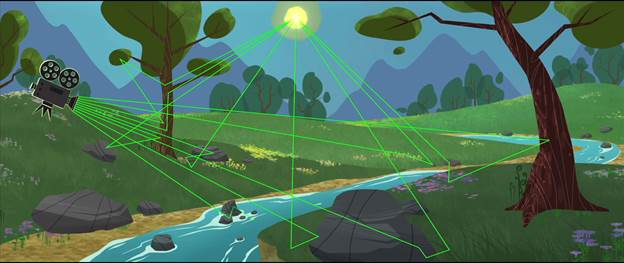
\includegraphics[width=0.85\textwidth]{images/ray_tracing.png}
\caption{Exemplo simplificado da aplicação do Ray Tracing.}
\label{figura:raytracing}
\end{figure}


\section{Relação com Outras Disciplinas do Curso de Ciência da Computação}
\paragraph{}

O perfil curricular do curso de Ciência da Computação exige a disciplina de 
Álgebra Vetorial e Linear para Computação como pré-requisito para seis cadeiras: IF680- Processamento Gráfico (obrigatória), F764- Cálculo Avançado para Computação (eletiva), IF109- Métodos Numéricos (eletiva), IF797- Otimização (eletiva), IF753- Processamento de sinais (eletiva) e IF777- Tópicos Avançados da Matemática Computacional (eletiva).Logo, nota-se que a Álgebra Vetorial e Linear para Computação está intimamente relacionada com diversas áreas do curso. \citep{Perfil}

\bibliographystyle{plain}
\bibliography{referencias}
\end{document}